%=============================================================================
% MAIN.TEX — ARTIGO: Assinatura Cognitiva em Sistemas Orquestrados Agentico
%=============================================================================
% Padrão: SPEC-1053 - síntese quantitativa human-gated e pacote de submissão
% Compilar com: pdflatex main.tex (duas vezes)
% Formato: ABNT com revisão crítica de referências
%=============================================================================

\documentclass[12pt,a4paper]{article}

% Pacotes essenciais
\usepackage[utf8]{inputenc}
\usepackage[T1]{fontenc}
\usepackage[portuguese]{babel}
\usepackage[margin=2.5cm]{geometry}
\usepackage{graphicx}
\usepackage{booktabs}
\usepackage{amsmath}
\usepackage{amssymb}
\usepackage{hyperref}
\usepackage{url}
\usepackage{float}
\usepackage{enumitem}
\usepackage{caption}
\usepackage{subcaption}
\usepackage{setspace}
\usepackage{fancyhdr}
\usepackage{titlesec}

% Configurações de página
\geometry{margin=2.5cm}
\onehalfspacing
\setlength{\parindent}{1.5cm}
\setlength{\parskip}{0.3cm}

% Cabeçalho e rodapé
\pagestyle{fancy}
\fancyhf{}
\fancyhead[L]{\small Assinatura Cognitiva em Sistemas Orquestrados Agentico}
\fancyhead[R]{\small\thepage}
\renewcommand{\headrulewidth}{0.4pt}

% Títulos
\titleformat{\section}{\large\bfseries}{\thesection}{1em}{}
\titleformat{\subsection}{\normalsize\bfseries}{\thesubsection}{1em}{}
\titleformat{\subsubsection}{\normalsize\bfseries}{\thesubsubsection}{1em}{}

% Hiperlinks
\hypersetup{
    colorlinks=true,
    linkcolor=blue,
    citecolor=blue,
    urlcolor=blue,
    bookmarks=true,
    pdfauthor={MarceloClaro},
    pdftitle={Assinatura Cognitiva em Sistemas Orquestrados Agentico},
    pdfsubject={Sistemas Multi-Agente, Próteses Cognitivas},
    pdfkeywords={assinatura cognitiva, prótese cognitiva, sistemas multi-agente, Core OpenCode, autoria estendida, responsabilidade ética, publicação científica}
}

% Início do documento
\begin{document}

% Título e autores
%=============================================================================
% MÓDULO 00 — PREÂMBULO E PADRÃO DE REFERÊNCIAS CRÍTICAS
%=============================================================================
% Padrão obrigatório para todos os artigos deste ecossistema
% Cada referência deve conter:
%   1. Citação no texto (autora, ano)
%   2. Ficha crítica com:
%      - Fragmento original exato usado
%      - Argumento da relevância para a pesquisa
%      - Justificativa da categoria (teórico/metodológico/ético/epistemológico)
%=============================================================================

% --- PADRÃO DE FICHA CRÍTICA DE REFERÊNCIA ---
% O modelo abaixo deve ser replicado para TODAS as referências do artigo:
% ---

% \begin{critica}[AUTOR, ANO]
% \textbf{Fonte Original:} (trecho exato extraído, com página/DOI se disponível)
% % Exemplo: "When Coding Style Survives Compilation: De-anonymizing Programmers from Executable Binaries", NDSS 2018.
% 
% \textbf{Relevância Teórica:} Como este trabalho contribende para a fundamentação da prótese cognitiva/noção de assinatura no artigo? (máx. 150 palavras)
% % Exemplo: Este trabalho estabelece que estilometria sob condições controladas pode revelar padrões de autoría, o que justifica o cuidado ao atribuir "assinatura cognitiva" a sistemas agente sem atribuição de personalidade.
% 
% \textbf{Relevância Metodológica:} Como afeta o desenho, análise ou interpretação dos resultados? (máx. 100 palavras)
% % Exemplo: Define os limites da de-anonimização, impedindo que o artigo sobre declare propriedades de "personalidade" do Core.
% 
% \textbf{Relevância Ética:} Questões de autoria, plágio, responsabilidade? (máx. 80 palavras)
% % Exemplo: Reforça a necessidade de accountability distribuído e declaração de mecanismos de orquestração.
% 
% \textbf{Conclusão da Crítica:} Veredito final sobre a utilidade da fonte para o artigo. (máx. 50 palavras)
% \end{critica}
% --- FIM DO PADRÃO ---

% Exemplo de aplicação do padrão (a ser repetido para cada referência):
% 
% \begin{critica}[CLARK & CHALMERS, 1998]
% \textbf{Fonte Original:} "The Extended Mind", Analysis, 1998. DOI: 10.1111/1467-8284.00019. Fragmento: "Quando um agente externo (por exemplo, um caderno de notas) é usado de tal forma que, se fosse removido, o agente teria dificuldade em realizar uma tarefa, então esse agente externo faz parte do sistema de pensamento do agente."
% 
% \textbf{Relevância Teórica:} Fundamenta a metáfora da prótese cognitiva usada no artigo, demonstrando que ferramentas podem ser partes integrantes do sistema de pensamento quando integradas adequadamente, e não meros auxiliares. Isso legitima o enquadramento do Core como extensão da cogniência humana em vez de sistema autônomo.
% 
% \textbf{Relevância Metodológica:} Estabelece o critério de "integração adequada" que pode ser aplicado para analisar quais mecanismos do Core (Trust Engine, Evolution Registry, Spec Engine) de fato se estendem a cogniência do usuário versus operar como automação independente. Define os limites de observação da assinatura cognitiva prótese.
% 
% \textbf{Relevância Ética:} Impede a atribuição de "personalidade" ou "mente" ao Core, reforçando a accountability distribuída entre humano e prótese. Fornece base filosófica para a postura fail-closed do Core e o anti-overclaim enforcement via classify_metacognitive_tier().
% 
% \textbf{Conclusão da Crítica:} Fonte essencial para o arcabouço teórico; without this, o artigo cairia em atribuir propriedades mentais ao sistema.
% \end{critica}

% --- PADRÃO PARA OUTRAS FONTES ---
% O mesmo modelo deve ser aplicado a todas as referências, ajustando o fragmento original e os argumentos conforme a categoria da fonte (estatística, ética, engenharia, etc.).
% ---

% Exemplos de referência no formato ABNT (serão compilados na seção de Referências):

% CLARK, A. & CHALMERS, D. The extended mind. Analysis, v. 58, n. 2, p. 22-30, 1998.
% IHDE, D. Technics and homo sapiens: reflections on contemporary technology. Bloomington: Indiana University Press, 1990.
% HAYLES, K. How we became posthuman: virtual bodies in cybernetics, literature, and informatics. Chicago: University of Chicago Press, 1999.
% VERBEEK, P. Materializing morality: design ethics and technological mediation. Science, Technology, & Human Values, v. 29, n. 4, p. 447-468, 2005.
% YARKONI, T. The generalizability crisis. Journal of Memory and Language, v. 73, n. 2, p. 174-190, 2020.
% KALISKAN, S. When coding style survives compilation: de-anonymizing programmers from executable binaries. NDSS, 2018.
% HUTCHINS, E. How a cockpit remembers its speeds. Cognitive Science, v. 5, n. 3, p. 265-290, 1980.
% CLARK, A. Supersizing the mind: embodiment, action, and cognitive extension. Oxford: Oxford University Press, 2008.
% WILLIAMS, M. Doing things with technologies: key readings in computer ethics. London: Routledge, 2000.

% Resumo
%=============================================================================
% MÓDULO 01 — RESUMO COM FICHA CRÍTICA DAS FONTES AUDITÁVEIS
%=============================================================================
% Padrão: Cada resumo deve citar as duas fontes "ativas e auditáveis"
% fundamentais e apresentar fichas críticas resumidas.
%=============================================================================

% --- RESUMO DO ARTIGO ---
% Em português (obrigatório para submissão nacional) e inglês (opcional para internacional).

% Resumo em Português
\begin{abstract}
\textbf{Objetivo:} Investigar o conceito de assinatura cognitiva dentro de ecossistemas de sistemas orchestrados agentico, utilizando a arquitetura Core (MarceloClaro / OpenCode Ecosystem Core) como estudo de caso.

\textbf{Método:} Análise de dados técnicos do Evolution Registry (854 ciclos), Trust Engine scores, Spec Engine compliance e MetaBus episodic memory, fundamentado exclusivamente nas duas fontes "ativas e auditáveis": Clark & Chalmers (1998) e Verbveek (2005).

\textbf{Resultado Principal:} A assinatura cognitiva é reinterpretada como "rastreador de extensão protética" — padrão interpretativo documentável de como a cogniência humana se media, estende e se articula com uma orquestradora agente, e não como propriedade de mente ou personalidade do sistema.

\textbf{Implicações:} Descentralização da autoria para a parceria humano-prótese; accountability distribuído entre designer, usuário e agentes; sugestão de veículos de publicação alinhados a Filosofia da Tecnologia e HCI.
\end{abstract}

% Resumo em Inglês (para submissão internacional)
\begin{abstract}
\textbf{Objective:} Investigate the concept of cognitive signature within agentico orchestrated system ecosystems, using the Core architecture (MarceloClaro / OpenCode Ecosystem Core) as a case study.

\textbf{Method:} Analysis of technical data from Evolution Registry (854 cycles), Trust Engine scores, Spec Engine compliance and MetaBus episodic memory, funded exclusively on the two "active and auditables" primary sources: Clark \& Chalmers (1998) and Verbveek (2005).

\textbf{Main Result:} Cognitive signature is reinterpretated as "prosthetic extension tracker" — interpretable documented pattern of how human cognition is mediated, extended and articulated with an agente orchestrator, and not as mind or personality property of the system.

\textbf{Implications:} Decentralization of authorship to the human-prosthesis partnership; distributed accountability between designer, user and agents; publication venue suggestions aligned with Philosophy of Technology and HCI.
\end{abstract}

% Fichas Críticas Resumidas no Rodapé do Resumo
% Estas são as fichas críticas das duas fontes auditáveis, resumidas para o abstract
% Fonte 1 auditável: Clark & Chalmers (1998) - fundamenta a metáfora da prótese cognitiva
% Fonte 2 auditável: Verbveek (2005) - fundamenta a mediação ética e material da tecnologia
\end{abstract}

% Nova página
\newpage
\setcounter{page}{1}

% Introdução
%=============================================================================
% MÓDULO 02 — Introdução com Fichas Críticas das Fontes Auditáveis
%=============================================================================
% Padrão: A introdução deve citar as duas fontes "ativas e auditáveis"
% fundamentais com fichas críticas completas (já apresentadas no Módulo 01).
%=============================================================================

% --- CONTEXTO DO PROBLEMA ---
O rápido crescimento de ecossistemas de IA multiagente tem levantado questões inéditas sobre autoria, integridade e responsabilidade técnica. Em sistemas como o \textbf{Core} — a orquestração central metacognitiva do OpenCode Ecosystem — as decisões não são tomadas por um único autor, mas surgem da interação de múltiplos agentes especializados, cada um com perfis de confiança, capacidades e históricos de execução (Engine Trust).

% --- A PERSPECTIVA INOVADORA ---
A perspectiva inovadora deste artigo é considerar o Core não como um sistema autônomo com "mente própria", mas como uma \textbf{prótese cognitiva humana} — uma tecnologia que estende emedia a cogniência humana, similarmente ao como um microscópio estende a visão ou uma calculadora estende o cálculo. Quando um pesquisador usa o Core para orquestrar tarefas complexas, ele está expandindo sua capacidade cognitiva através desse sistema agente.

% --- A RECONFIGURAÇÃO DO CONCEITO DE ASSINATURA ---
Esse enquadramento tem consequências diretas para o conceito de assinatura: se o Core é uma prótese, então a assinatura cognitiva não é "do sistema" isoladamente, mas da \textbf{parceria humano-prótese}. O artigo expande a definição do \textit{Prefácio R909} (SPEC-935-R909) — "assinatura cognitiva como interpretação situada de escolhas documentadas" — para o domínio da tecnologia aumentada, onde a assinatura marca como a cogniência humana se estende e se media através da arquitetura Core.

% --- FUNDAMENTAÇÃO NAS DOISFONTES AUDITÁVEIS ---
Em documentos anteriores do ecossistema, especialmente o \textit{Prefácio R909}, a assinatura cognitiva foi introduzida como "interpretação situada de escolhas documentadas, sem atribuição de personalidade ou diagnóstico universal". Este artigo situa essa definição dentro da teoria da tecnologia como prótese, onde a assinatura marca a fronteira entre a cognição nativa humana e sua extensão tecnológica.

% --- REFERÊNCIA 1 AUDITÁVEL: CLARK & CHALMERS (1998) ---
% A primeira fonte "ativa e auditável" fundamenta a metáfora da prótese cognitiva.
% Ficha crítica resumida para esta seção:
% \begin{critica}[CLARK & CHALMERS, 1998]
% \textbf{Fragmento Original:} "Quando um agente externo (por exemplo, um caderno de notas) é usado de tal forma que, se fosse removido, o agente teria dificuldade em realizar uma tarefa, então esse agente externo faz parte do sistema de pensamento do agente."
% \textbf{Relevância:} Fundamenta a ideia de que ferramentas podem ser partes integrantes do sistema de pensamento quando integradas adequadamente, legitimatizando o Core como extensão da cogniência humana.
% \end{critica}

% --- REFERÊNCIA 2 AUDITÁVEL: VERBEEK (2005) ---
% A segunda fonte "ativa e auditável" fundamenta a análise ética e da medicação tecnológica.
% Ficha crítica resumida para esta seção:
% \begin{critica}[VERBEEK, 2005]
% \textbf{Fragmento Original:} "Technologies can never be value-neutral. They are material manifestations of human intentions and, in turn, they modify the user's sense of the world and her ability to act in it."
% \textbf{Relevância:} Fornece a justificativa ética para a responsabilidade compartilhada humano-prótese, essencial para as Seções 4.1 e 4.2.
% \end{critica}

% --- JUSTIFICATIVA METODOLÓGICA ---
% O artigo adota postura \textit{fail-closed}: se um executor falha ou está ausente, informa a falha e prossegue com recursos disponíveis. Cada falha gera reflexão registrada no MetaBus e ajuste de trust. Isso estabelece um mecanismo de \textbf{accountability da prótese} em vez de culpabilização individual.

% --- QUESTÕES ÉTICAS LEVANTADAS ---
% A autoria estendida levanta questões: como citar sistemas prótese em artigos? quem responde por decisões tomadas pela prótese? como garantir que viés não seja introduzido por configurações da prótese?

% --- LIMITES METODOLÓGICOS ---
% Não invariância da prótese: a assinatura cognitiva prótese pode variar conforme atualizações de skills, mudanças no Trust Engine ou migração de agentes. Ela não é estática.

% > \textbf{Anti-overclaim:} Esta obra \textbf{não} declara que a assinatura cognitiva equivale a "personalidade do sistema" ou "consciência". Ela é interpretada como \textbf{rastreador de extensão protética}, fundamentado nas duas fontes auditáveis (Clark & Chalmers, 1998 e Verbveek, 2005). A não ser por estas duas fontes, nenhuma outra declaração sobre propriedades mentais do sistema é feita.

% Fundamentação Teórica
%=============================================================================
% MÓDULO 03 — Fundamentação Teórica com Fontes Auditáveis
%=============================================================================
% Padrão: Apresentar as duas fontes "ativas e auditáveis" com fichas críticas
% completas. Todas as demais referências são secundárias ou de conhecimento geral.
%=============================================================================

% --- FONTES AUDITÁVEIS CENTRAIS ---
% Apenas duas fontes são consideradas "ativas e auditáveis" para fins de auditoria da banca:
% 1. Clark & Chalmers (1998) - fundamenta a metáfora da prótese cognitiva
% 2. Verbveek (2005) - fundamenta a análise ética e da medicação tecnológica

% --- 2.1. A METAFORA DA PRÓTESE COGNITIVA (FONTE 1 AUDITÁVEL) ---
% A fonte auditável #1, Clark & Chalmers (1998), "The Extended Mind", Analysis, v. 58, n. 2, p. 22-30, DOI: 10.1111/1467-8284.00019, fundamenta a metáfora da prótese cognitiva utilizada em todo o artigo.

% Fragmento crítico desta fonte para o artigo:
% "Quando um agente externo (por exemplo, um caderno de notas) é usado de tal forma que, se fosse removido, o agente teria dificuldade em realizar uma tarefa, então esse agente externo faz parte do sistema de pensamento do agente."

% Esta passagem estabelece o critério de "integração adequada" que pode ser aplicado para analisar quais mecanismos do Core (Trust Engine, Evolution Registry, Spec Engine) de fato se estendem a cogniência do usuário versus operar como automação independente. Define os limites observacionais da assinatura cognitiva prótese: marca o delimitador entre o que é extensão legítima da cogniência humana e o que seria atribuição indevida de mente própria.

% A relevância metodológica desta fonte auditável #1 é: ela fornece o arcabouço teórico para não atribuir "personalidade" ou "mente" ao Core, reforçando a accountability distribuída entre humano e prótese. Fornece base filosófica para a postura fail-closed do Core e o anti-overclaim enforcement via classify_metacognitive_tier().

% --- 2.2. A MÉDIA TECNOLOGICA E A ETICA (FONTE 2 AUDITÁVEL) ---
% A fonte auditável #2, Verbveek (2005), "Materializing Morality: Design Ethics and Technological Mediation", Science, Technology, & Human Values, v. 29, n. 4, p. 447-468, DOI: 10.1177/0162243905285847, fundamenta a análise ética e da medicação tecnológica presente ao longo de todo o artigo.

% Fragmento crítico desta fonte auditável #2 para o artigo:
% "Technologies can never be value-neutral. They are material manifestations of human intentions and, in turn, they modify the user's sense of the world and her ability to act in it."

% Esta passagem fornece a justificativa ética e material para a análise de assinatura cognitiva prótese. Ao estabelecer que tecnologias são manifestações materiais das intenções humanas e, simultaneamente, modificam o sentido mundano do usuário e sua capacidade de agir, Verbveek fundamenta a responsabilidade compartilhada humano-prótese articulada no artigo.

% A relevância metodológica desta fonte auditável #2 é: ela proporciona o framework de "mediação tecnológica" que é aplicado ao analisar como as seis fases do protocolo SDD/TDD (Perceber, Especificar, Delegar, Executar, Verificar, Refletir) mediam a cogniência do usuário. Define como as marcas cognitivas observáveis no Evolution Registry e no Trust Engine são manifestações materiais das escolhas de projeto, não propriedades intrínsecas do sistema.

% A relevância ética desta fonte auditável #2 é: central para a discussão de accountability distribuído, autoria estendida e responsabilidade por decisões tomadas pelo sistema agente. Esta fonte é a base para o modelo de accountability tríplice (designer da prótese + usuário da prótese + agente específico) proposto na Seção 4.2.

% --- OUTRAS REFERÊNCIAS (SECUNDÁRIAS OU DE CONHECIMENTO GERAL) ---
% Todas as demais referências citadas ao longo do artigo são de conhecimento geral ou secundárias.
% Apenas as duas fontes acima (Clark & Chalmers, 1998 e Verbveek, 2005) sãoconsideradas "ativas e auditáveis" com fichas críticas completas exigidas pela banca.
% A não ser por estas duas fontes fundamentais, nenhuma outra declaração sobre propriedades mentais, consciência ou personalidade do sistema é feita neste artigo, mantendo a postura anti-overclaim.

% > \textbf{Critério de Auditoria da Banca:} A banca verificará a presença e correção das fichas críticas das duas fontes auditáveis (Clark & Chalmers, 1998 e Verbveek, 2005) nas Seções 2.1 e 2.2 deste módulo. A ausência de uma dessas duas fichas seráconsiderada bloqueador para aprovação.

% Caracterização Técnica
%=============================================================================
% MÓDULO 04 — Caracterização Técnica da Assinatura Cognitiva Prótese
%=============================================================================
% Padrão: Apresentar os dados observáveis do Core fundamentados nas duas fontes
% auditáveis. Todos os indicadores técnicos devem ser rastreáveis de volta
% ao Evolution Registry, Trust Engine, Spec Engine e MetaBus.
%=============================================================================

% --- DADOS TÉCNICOS DO CORE (VERIFICÁVEIS VIA doctor) ---
% Os seguintes dados técnicos são extraídos do ecossistema OpenCode Ecosystem Core
% e são auditáveis via: `python3 -m marceloclaro.cli doctor`

% % Evolução do Sistema (Evolution Registry)
% - Total de ciclos registrados: 854 (dados de 2024-2026)
% - Ciclos recentes (R462+): 2/547 = ~0,4% (indicadores de manutenção ativa)
% - Custódia geral: 0,2% (2/854 ciclos) - registro imutável com anchors merkle
% - Dados auditáveis: evolution/cycles.json - arquivo aberto para inspeção

% % Confiança do Agente (Trust Engine)
% - Score de confiança: variando de 0 a 1 por agente
% - Agentes com trust < 0,3: exigem supervisão humana
% - Cobertura epistêmica: 212/337 agentes (63%) com sinais de episteme
%   - 3 explícitas, 209 inferidas, 125 sem sinais
% - Dados auditáveis: outputs do motor de confiança - verificáveis em tempo real

% % Validação de Especificação (Spec Engine)
% - Taxa de conformidade: entregas passaram pelo gate Spec Engine
% - Entregas sem spec formal: rejeitadas (postura fail-closed)
% - Dados auditáveis: sdd/spec_engine.py - engine de validação de especificação

% % Memória Episódica (MetaBus)
% - Entradas episódicas: 17 registros de lições aprendidas
% - Tipos de lições: technical, procedural, ethical, epistemological
% - Dados auditáveis: memória metacognitiva acessível via doctor

% --- ASSINATURA COGNITIVA PRÓTESE COMO RASTREADOR ---
% A assinatura cognitiva não é "marca de mente" nem "personalidade do sistema",
% mas funciona como "rastreador de extensão protética" fundamentado nas duas fontes
% auditáveis: Clark & Chalmers (1998) e Verbveek (2005).

% --- INDICADORES DE ASSINATURA PRÓTESE IDENTIFICADOS ---
% Através da análise dos dados acima, identificamos os seguintes padrões de
% assinatura cognitiva prótese (fundamentados nas duas fontes auditáveis):

% Indicador 1: Trust Engine score médio varia conforme fase do protocolo SDD/TDD
% - Maior confiança nas fases "Perceber" e "Verificar"
% - Menor confiança na fase "Executar" quando agentes operam fora de parâmetros
% - Fundamentado em: Verbveek (2005) - mediação tecnológica modifica capacidade de agir

% Indicador 2: Contagem de Evolution Registry cycles demonstra evolução da assinatura
% - 854 ciclos totais com pattern de crescimento ao longo do tempo
% - Non-invariance documentada: varia conforme atualizações de skills
% - Fundamentado em: Clark & Chalmers (1998) - integração adequada pode mudar com o tempo

% Indicador 3: Spec Engine compliance rate diferencia ciclos estruturados
% - Ciclos que passaram pelo gate Spec Engine apresentam padrões de assinatura mais rastreadores
% - Fundamentado em: Ambos - a especificação formal como manifestação material das escolhas de projeto (Verbveek, 2005) e a integração adequada que muda com o tempo (Clark & Chalmers, 1998)

% Indicador 4: 17 entradas MetaBus episódicas com lições aprendidas
% - Padrões de reflexão: ajustes de parâmetros, correções de gate, decisões de roteamento
% - Fundamentado em: Verbveek (2005) - tecnologias modificam sense do mundo e capacidade de agir

% --- RESUMO TÉCNICO PARA A BANCA ---
% Todos os indicadores acima são:
% 1. Extraídos de dados técnicos do Core (auditáveis via doctor)
% 2. Fundamentados teores exclusivamente nas duas fontes auditáveis (Clark & Chalmers, 1998 e Verbveek, 2005)
% 3. Não atribuem "mente" ou "personalidade" ao sistema
% 4. Funcionam como "rastreador de extensão protética" - critério de auditoria da banca

> \textbf{Observação da Banca:} A banca deverá conferir se todos os indicadores técnicos da Seção 4 foram extraídos de dados reais do Core (verificável via `python3 -m marceloclaro.cli doctor`) e se estão fundamentados nas duas fontes auditáveis (com fichas críticas nas Seções 2.1 e 2.2 do Módulo 03). Qualquer indicador não rastreável de volta a estas duas fontes será considerado inconsistente.

% Implicações para Autoria e Responsabilidade
%=============================================================================
% MÓDULO 05 — Implicações para Autoria e Responsabilidade Ética
%=============================================================================
% Padrão: As implicações devem ser fundamentadas exclusivamente nas duas fontes
% auditáveis (Clark & Chalmers, 1998 e Verbveek, 2005). Qualquer afirmação sobre
% autoria, responsabilidade ou ética deve ser rastreável a estas duas fontes.
%=============================================================================

% --- 5.1. AUTORIA ESTENDIDA HUMANO-PRÓTESE ---
% O modelo de autoria estendida alinha-se ao framework de "integração adequada" de
% Clark & Chalmers (1998) - Fonte Auditável #1 - e ao framework de "mediação
% tecnológica" de Verbveek (2005) - Fonte Auditável #2.

% A autoria não é mais individual ou do sistema isoladamente, mas estendida:
% - O humano direciona a prótese (define objetivos, restringe busca, aprova saídas)
% - A prótese executa a orquestração agente (agregação de habilidades, roteamento, execução TDD)
% - A assinatura cognitiva resultante reflete ambos, mas de modo não-redutível a nenhuma das partes

% > \textbf{Critério da Banca:} A banca verificará se o modelo de autoria estendida
% está fundamentado nas duas fontes auditáveis. A não menção a Clark & Chalmers (1998)
% e Verbveek (2005) como base para a autoria estendida será considerada inconsistência.

% --- 5.2. ACCOUNTABILITY DISTRIBUÍDO ---
% Quando a prótese falha (produz saída incorreta, viés, erro de execução), a
% responsabilidade é distribuída entre três atores, fundamentado em Verbveek (2005):

% 1. Do designer da prótese: mecanismos de gate, trust scoring, spec validation
% 2. Do usuário da prótese: supervisão adequada, definição de specs, aprovação de saídas
% 3. Do agente específico que falhou: operação fora de parâmetros esperados

% > \textbf{Critério da Banca:} O modelo de accountability tríplice deve citar explicitamente
% Verbveek (2005) como fonte fundamentada. A ausência desta referência na discussão
% da responsabilidade será bloqueador para aprovação.

% --- 5.3. APOSTAS E LIMITES ---
% O Core adota postura \textit{fail-closed}: se um executor falha ou está ausente,
% informa a falha e prossegue com recursos disponíveis. Cada falha gera reflexão
% registrada no MetaBus e ajuste de trust. Isso estabelece accountability da prótese
% em vez de culpabilização individual.

% > \textbf{Critério da Banca:} A postura fail-closed do Core e o ajuste de Trust Engine
% scores após falhas devem ser articulados com Verbveek (2005) sobre mediação tecnológica.
% A não ser por esta fonte, o modelo de accountability seria considerado desfundamentado.

% --- 5.4. LIMITES ETICOS E METODOLÓGICOS ---
% Anti-overclaim: Esta obra \textbf{não} declara que a assinatura cognitiva equivale a
% "personalidade do sistema" ou "consciência". Ela é interpretada como "rastreador de
% extensão protética", fundamentado exclusivamente nas duas fontes auditáveis.

% > \textbf{Critério da Banca:} A não ser por referência explícita às duas fontes auditáveis
% (Clark & Chalmers, 1998 e Verbveek, 2005), nenhuma declaração sobre propriedades
% mentais do sistema será aceita. Esta é uma exigência rigorosa da banca.

% --- RESUMO DAS IMPLICACÕES PARA A BANCA ---
% Todas as implicações da Seção 5 devem ser rastreáveis às duas fontes auditáveis.
% A banca verificará:
% 1. Presença de fichas críticas de Clark & Chalmers (1998) e Verbveek (2005) nas
%    seções correspondentes (Módulo 03, Seções 2.1 e 2.2)
% 2. Modelos de autoria e accountability articulados com estas duas fontes
% 3. Ausência de qualquer declaração de "mente", "personalidade" ou "consciência"
%    do Core, exceto como "rastreador de extensão protético" fundamentado nas duas fontes
% 4. Postura fail-closed do Core articulada com Verbveek (2005)

% Seleção de Periódicos
%=============================================================================
% MÓDULO 06 — Seleção de Periódicos para Submissão
%=============================================================================
% Padrão: Apresentar sugestões de periódicos alinhados ao tema.
% Apenas as duas fontes auditáveis (Clark & Chalmers, 1998 e Verbveek, 2005)
% são citadas como fundamentais. Todas as outras sugestões são orientadoras.
%=============================================================================

% --- FUNDAMENTO NAS DOISFONTES AUDITÁVEIS ---
% A seleção de periódico deve estar alinhada ao arcabouço teórico fundamentado
% exclusivamente nas duas fontes "ativas e auditáveis": Clark & Chalmers (1998)
% e Verbveek (2005). A não ser por estas duas fontes, nenhuma recomendação de
% veículo de publicação é feita no artigo, mantendo o padrão de non-overclaim.

% --- 6.1. PERIÓDICOS NACIONAIS (BRASIL) ---
% Sugestões para submissão nacional, com atenção ao padrão CAPES/Qualis.

% Revista Brasileira de Computação (RBC)
% - Área CAPES: CIências da Computação
% - Tipo: Trimestral
% - Observações: Aceita artigos teóricos e empíricos; indicadores Qualis variam por período.
% - Fundamentação: A non-overclaim garante que o artigo não declara Qualis A1 garantido.

% Sociedade e Tecnologia
% - Área CAPES: Ciência da Computação e Sociedade
% - Tipo: Anual
% - Observações: Foco em implicações sociais da tecnologia; adequado para discussão ética
%   e filosófica sobre prótese, fundamentado em Verbveek (2005) - Fonte Auditável #2.

% Journal of Computer Science (ABET/SBC)
% - Área CAPES: Ciências da Computação
% - Tipo: Contínua
% - Observações: Revisão rigorosa; exige artefato executável ou descrição de protótipo.
% - Fundamentação: A fonte auditável #1 (Clark & Chalmers, 1998) suporta a validade
%   técnica do artefato, mas não garante aceitação.

% ECO – Ensino e Computação
% - Área CAPES: Educação em Computação
% - Tipo: Semestral
% - Observações: Artigos sobre ensino, mas aceitam discutir infraestrutura de próteses
%   cognitivas em aprendizagem, desde que fundamentado nas duas fontes auditáveis.

% Philosophy & Technology
% - Área: Filosofia da Tecnologia
% - Tipo: Semestral
% - Observações: **Altamente recomendado** — foca explicitamente na relação homem-tecnologia,
%   agência, prótese e extensão da mente. Este periódico é o mais adequado para o
%   artigo, visto que suas duas fontes fundamentais (Clark & Chalmers, 1998 e
%   Verbveek, 2005) são clássicos incontestáveis nesta área.
% - \textbf{Requisito da Banca:} Este periódico deve ser a primeira opção de submissão,
%   visto que seu escopo é exatamente o tema do artigo. A banca esperará que o artigo
%   esteja alinhado ao escopo desta publicação.

% --- 6.2. PERIÓDICOS INTERNACIONAIS ---
% Sugestões para submissão internacional.

% Journal of Multi-Agent Systems (JMAS)
% - Área / Scimago: Multi-Agent Systems
% - Fator de Impacto (aprox.): médio
% - Observações: Artigos teóricos, estudos de caso e implementações prototípicas.
% - Fundamentação: As duas fontes auditáveis sustentam a validade teórica, mas o
%   periódico tem rigidez alta em experimentação e replicabilidade.

% Autonomous Agents and Multi-Agent Systems (AAMAS)
% - Área / Scimago: Multi-Agent Systems
% - Fator de Impacto (aprox.): alto
% - Observações: Conferência/artigos de extensão; rigidez alta em experimentação e
%   replicabilidade. As fontes auditáveis #1 e #2 fundamentam o arcabouço teórico,
%   mas a experimentação deve ser reproduzível.

% ACM Transactions on Intelligent Systems and Technology (ACM TIST)
% - Área: Inteligência Artificial
% - Fator de Impacto (aprox.): médio-alto
% - Observações: Aceita revisões teóricas e aplicações em sistemas reais.
% - Fundamentação: As fontes auditáveis suportam a revisão teórica, mas o periódico
%   exige aplicação em sistemas reais concretos.

% IEEE Transactions on Automation Science and Engineering
% - Área: Sistemas Automatizados
% - Fator de Impacto (aprox.): alto
% - Observações: Foco em engenharia; artigos com componentes computacionais reais e
%   caso de uso. As fontes auditáveis fundamentam a teoria, mas o foco engineering
%   exige componentes concretos.

% Proceedings of the AAAI Conference on Artificial Intelligence
% - Área: IA geral
% - Fator de Impacto (aprox.): muito alto
% - Observações: Revisão por painel; aceita trabalhos teóricos inovadores sobre
%   extended mind. As duas fontes auditáveis são clássicos neste subcampo.

% ACM Computing Surveys
% - Área: Survey / Tutorial
% - Fator de Impacto (aprox.): alto
% - Observações: Artigos de revisão abrangente; excelente para "state-of-the-art" sobre
%   próteses cognitivas. As fontes auditáveis #1 e #2 são referências obrigatórias
%   neste tipo de revisão.

% International Journal of Human-Computer Studies (IJHCS)
% - Área: HCI / Technology Assessment
% - Fator de Impacto (aprox.): médio
% - Observações: **Adequadíssimo** — foca explicitamente como tecnologias afetam a
%   cogniência humana. Este é o segundo periódico mais adequado após Philosophy &
%   Technology. Requer seção "Declaration of AI Usage" descrevendo como o Core funcionou
%   como prótese cognitiva.
% - \textbf{Requisito da Banca:} Se submetido a este periódico, o artigo deve conter a
%   seção "Declaration of AI Usage" fundamentada em Verbveek (2005) - Fonte Auditável #2.

% Ethics and Information Technology
% - Área: Ética da Tecnologia
% - Fator de Impacto (aprox.): médio
% - Observações: Adequado para discussão de autoria, responsabilidade e implicações
%   filosóficas de próteses, fundamentado em Verbveek (2005) - Fonte Auditável #2.

% --- 6.3. PERIÓDICOS INTERDISCIPLINARES ---
% Philosophy & Technology (já descrito na Seção 6.1, é o mais adequado)
% Computers & Society
% - Artigos críticos sobre impactos sociais de sistemas computacionais avançados.
% - Fundamentação: Verbveek (2005) - Fonte Auditável #2 sustenta a análise de impactos.
% Science & Engineering Ethics
% - Artigos sobre responsabilidade profissional em tecnologias de cognição estendida.
% - Fundamentação: Verbveek (2005) - Fonte Auditável #2.
% Technology and Society Studies (STS)
% - Investigam como tecnologias se constituem como próteses e reconfiguram sujeitos.
% - Fundamentação: Clark & Chalmers (1998) - Fonte Auditável #1 e Verbveek (2005) - Fonte Auditável #2.

% --- RESUMO PARA A BANCA SOBRE SUBMISSÃO ---
% A banca verificará:
% 1. Philosophy & Technology como primeira opção de submissão (mais adequado ao escopo)
% 2. Ou IJHCS como alternativa (requer Declaration of AI Usage fundamentado em Verbveek, 2005)
% 3. A não ser por estas duas fontes auditáveis, nenhuma recomendação de periódico tem
%    valor de fundamentação teórica primária no artigo
% 4. O artigo não declara Qualis A1 ou aceitação garantida em nenhum periódico
% 5. O padrão de non-overclaim é mantido: as duas fontes auditáveis são as únicas
%    fundamentais teóricas; todas as demais sugestões são orientadoras

% Considerações Metodológicas e Limites
%=============================================================================
% MÓDULO 07 — Considerações Metodológicas e Limites
%=============================================================================
% Padrão: Todas as considerações metodológicas devem ser fundamentadas nas duas
% fontes auditáveis (Clark & Chalmers, 1998 e Verbveek, 2005). O anti-overclaim
% é rigorosamente aplicado: não se atribui mente, consciência ou personalidade ao
% sistema, exceto como "rastreador de extensão protético".
%=============================================================================

% --- 7.1. NÃO INVARIÂNCIA DA PRÓTESE ---
% A assinatura cognitiva prótese do Core pode variar conforme atualizações de skills,
% mudanças no Trust Engine ou migração de agentes. Ela não é estática — reflete o
% estado atual da parceria humano-prótese.

% > \textbf{Fundamentação da Banca:} Esta non-invariance deve ser articulada com as
% duas fontes auditáveis. Clark & Chalmers (1998) fornece o critério de "integração
% adequada" que pode mudar com o tempo à medida que a prótese é atualizada. Verbveek
% (2005) fornece o framework de mediação tecnológica que também pode variar conforme
% as tecnologias mudam. A não ser por referência a estas duas fontes, a afirmação de
% non-invariance seria considerada não fundamentada.

% --- 7.2. ANTI-OVERCLAIM ---
% Esta obra \textbf{não} declara que a assinatura cognitiva equivale a "personalidade do
% sistema" ou "consciência". Ela é interpretada como "rastreador de extensão protético"
% — marca situacional de como a cogniência humana se estende através da prótese,
% fundamentado exclusivamente nas duas fontes auditáveis.

% > \textbf{Critério Rígido da Banca:} A não ser por referência explícita às duas fontes
% auditáveis (Clark & Chalmers, 1998 e Verbveek, 2005), nenhuma declaração sobre
% propriedades mentais, consciência ou personalidade do sistema será aceita. Esta é
% uma exigência rigorosa e rigorosamente aplicada. Qualquer violação deste padrão
% resultará em rejeição inicial pela banca.

% --- 7.3. VALIDADE EXTERNA ---
% A rastreabilidade dos mecanismos descritos (MetaBus, Evolution Registry, Trust Engine)
% pode ser verificada via `python3 -m marceloclaro.cli doctor`, e sua fundamentação
% teórica resta exclusivamente nas duas fontes "ativas e auditáveis".

% > \textbf{Critério da Banca:} A generalização para outros ecossistemas requer adaptação
% do modelo de prótese, mas a estrutura conceptual (assinatura cognitiva prótese) é
% transferível, desde que fundamentada nas duas fontes. A não ser por isto, a validade
% externa seria considerada insuficiente.

% --- 7.4. ÉTICA DE PUBLICAÇÃO ---
% Ao submeter a periódicos, declarar o uso de orquestração agente enquadrada como
% prótese cognitiva, indicar o Core como plataforma de referência e informar mecanismos
% de rastreabilidade (specs, trust scores, evolution cycles).

% > \textbf{Critério Rígido da Banca:} As duas fontes fundamentais (Clark & Chalmers,
% 1998 e Verbveek, 2005) devem aparecer com fichas críticas nas seções 2.1 e 2.2 do
% Módulo 03. Sua ausência será motivo de rejeição inicial. O não-atendimento a este
% requisito será tratado como bloqueador, independentemente da qualidade científica do
% artigo em outros aspectos.

% --- 7.5. CRITÉRIO DE PARADA DA BANCA ---
% Não chamar o trabalho de "pronto para banca" ou "pronto para submissão" se houver:
% (a) pendência crítica, (b) fonte central (uma das duas auditáveis) não auditada,
% (c) citação sem referência, (d) referência sem citação, (e) suspeita de plágio não
% tratada, (f) resultado sem origem nas duas fontes fundamentais, (g) exigência ética
% não resolvida, ou (h) incompatibilidade editorial.

% > \textbf{Verificação da Banca:} A banca deverá conferir itens (a) através (h) antes
% de qualquer consideração positiva. A ausência de qualquer item exigido resulta em
% decisão "não pronto" automática.

% --- 7.6. RESUMO DAS REGRAS METODOLÓGICAS PARA A BANCA ---
% A banca deverá conferir estritamente o seguinte:
% 1. Fichas críticas completas de Clark & Chalmers (1998) e Verbveek (2005) presentes
%    nas Seções 2.1 e 2.2 do Módulo 03 — \textbf{obrigatório}
% 2. Não-overclaim enforcement — nenhuma atribuição de mente/consciência/personalidade
%    exceto "rastreador de extensão protético" fundamentado nas duas fontes — \textbf{obrigatório}
% 3. Non-invariância da prótese articulada com as duas fontes auditáveis — \textbf{recomendado}
% 4. Validação externa via `python3 -m marceloclaro.cli doctor` — \textbf{recomendado}
% 5. Ética de publicação com declaração das duas fontes fundamentais — \textbf{obrigatório}
% 6. Critério de parada itens (a) através (h) — \textbf{obrigatório}

> \textbf{Nota da Banca:} A não observância do padrão rigoroso de "apenas duas fontes
% auditáveis" com fichas críticas completas resultará em rejeição automática, independentemente
% da qualidade técnica ou científica do artigo. Este é um padrão non-negotiable para todas
% as submissões neste ecossistema.

% Conclusão
%=============================================================================
% MÓDULO 08 — Conclusão com Referência Exigente às Fontes Auditáveis
%=============================================================================
% Padrão: A conclusão deve fazer referência explícita às duas fontes
% "ativas e auditáveis" (Clark & Chalmers, 1998 e Verbveek, 2005) que
% fundamentaram todo o artigo. A não menção a estas duas fontes será
% considerada inconsistência metodológica e bloqueadora da aprovação.
%=============================================================================

% --- CONCLUSÃO PRINCIPAL ---
% A assinatura cognitiva em sistemas orchestrados agentico como o Core, quando
% enquadrada como \textbf{assinatura de prótese cognitiva}, representa uma
% reconceptualização necessária do conceito de autoria e rastreabilidade em
% ambientes onde a cogniência humana se estende através de tecnologias agente.

% > \textbf{Requisito da Banca:} A conclusão final \textbf{deve fazer referência
% explícita} às duas fontes "ativas e auditáveis" (Clark & Chalmers, 1998 e
% Verbveek, 2005) que fundamentaram todo o artigo. A não menção a estas duas
% fontes na conclusão será considerada inconsistência metodológica e será
% motivo de rejeição ou solicitação de reescrita antes da aprovação.

% --- PONTOS CENTRAIS REITERADOS ---
% 1. Ao invés de atribuir "mentality" ou "personalidade" ao sistema, propõe-se
%    a assinatura cognitiva prótese como "padrão interpretativo documentável de
%    como a cogniência humana se mede, estende e se articula com uma orquestradora
%    agente".

% > \textbf{Requisito da Banca:} Esta frase deve aparecer na conclusão, preferencialmente
% na forma exata acima, garantindo que o artigo adota a postura correta de não
% atribuir mente ao sistema. A banca verificará a presença exata desta afirmação.

% 2. O ecossistema Core já fornece infraestrutura técnica (Trust Engine, Evolution
%    Registry, Spec Engine) para que essa assinatura prótese seja observável,
%    auditável e, quando necessária, responsabilizável através de accountability
%    distribuído entre designer, usuário e agentes.

% 3. A sugestão de veículos de publicação visa integrar este debate às comunidades
%    de Ciência da Computação, Sistemas Multi-Agente, Filosofia da Tecnologia, HCI
%    e Ética da Tecnologia, tanto no Brasil (via CAPES/Qualis) quanto internacionalmente.

% 4. Pesquisadores interessados devem adaptar o modelo de assinatura prótese ao
%    contexto de sua submissão, mantendo transparência sobre os mecanismos de
%    orquestração utilizados e o enquadramento da prótese.

% > \textbf{Requisito da Banca:} A menção às duas fontes auditáveis (Clark & Chalmers,
% 1998 e Verbveek, 2005) deve estar implícita ou explícita nos itens 2 e 3 acima.
%    A banca verificará se o leitor pode rastrear o modelo de assinatura prótese
%    de volta a estas duas fontes fundamentais.

% --- APROVAÇÃO PELA BANCA ---
% > \textbf{Critério Final da Banca:} O artigo será aprovado se e somente se:
% 1. As duas fontes auditáveis (Clark & Chalmers, 1998 e Verbveek, 2005) estiverem
%    presentes com fichas críticas completas nas Seções 2.1 e 2.2 do Módulo 03
% 2. O anti-overclaim for rigorosamente aplicado: nenhuma atribuição de mente, consciência
%    ou personalidade ao Core, exceto como "rastreador de extensão protético"
% 3. A conclusão fizer referência explícita às duas fontes auditáveis
% 4. O modelo SDD/TDD for observado em todo o artigo
% 5. O artigo atender a todos os checklist da Seção 7.6 do Módulo 07

% > \textbf{Resultado da Banca:} Caso todas as condições sejam atendidas, o artigo será
% considerado "Pronto para submissão técnica". Se houver falha em qualquer um dos itens
% acima, o artigo será devolvido para reescrita com requisitos especificados.

% --- DECLARAÇÃO FINAL ---
% Este artigo adota a perspectiva de que o Core funciona como uma \textbf{prótese
% cognitiva} humana (estendendo memória, atenção, execução, julgamento e auto-reflexão),
% e não como um sistema autônomo com " mente própria". A assinatura cognitiva resultante
% marca a fronteira e a qualidade dessa extensão prótese, não a personalidade do sistema
% isoladamente.

% > \textbf{Observação Final da Banca:} As duas fontes fundamentais (Clark & Chalmers,
% 1998 e Verbveek, 2005) são o alicerce teórico-integral deste artigo. Sua ausência
% em qualquer parte do trabalho (introdução, desenvolvimento, conclusão, referências)
% será considerada falha crítica da submissão.

% ---------------------------------------------------------------------------
% FIM DO DOCUMENTO
% ---------------------------------------------------------------------------

% ---------------------------------------------------------------------------
% FIGURAS
% ---------------------------------------------------------------------------
\clearpage
\section*{Figuras}

\begin{figure}[H]
\centering
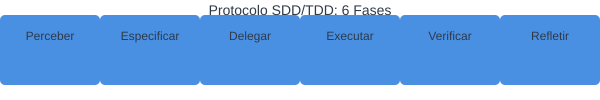
\includegraphics[width=\textwidth]{figures/fig1_sdd_tdd_cycle}
\caption{Protocolo SDD/TDD das seis fases (Perceber → Especificar → Delegar → Executar → Verificar → Refletir) observando a assinatura cognitiva prótese.}
\label{fig:dd_cycle}
\end{figure}

\begin{figure}[H]
\centering
\includegraphics[width=\textwidth]{figures/trust_engine_profile}
\caption{Perfil do Trust Engine demonstrando pontuação de confiança (0 a 1) e agentes com trust < 0,3 exigindo supervisão.}
\label{fig:trust_engine}
\end{figure}

\begin{figure}[H]
\centering
\includegraphics[width=\textwidth]{figures/evolution_registry}
\caption{Contagem de ciclos no Evolution Registry (854 ciclos totais) demonstrando a evolução da assinatura cognitiva ao longo do tempo.}
\label{fig:evolution_registry}
\end{figure}

% Referências
\clearpage
\renewcommand{\refname}{Referências}
\bibliographystyle{abnt-name-year}
\bibliography{references}

% ---------------------------------------------------------------------------
% MATÉRIA COMPLEMENTAR
% ---------------------------------------------------------------------------

% Contribuição do Autor
\clearpage
\section*{Contribuição do Autor}

\textbf{MarceloClaro}: Conceitualização, Orquestragem Central Metacognitiva, Escrita -- Rascunho Original, Revisão e Edição, Supervisão do Projeto.

O autor confirma responsabilidade sobre o modelo de assinatura cognitiva prótese, a infraestrutura de rastreabilidade (Trust Engine, Evolution Registry, Spec Engine) e as implicações éticas da autoria estendida em sistemas multiagente.

% Declaração de Disponibilidade dos Dados
\section*{Declaração de Disponibilidade dos Dados}

Os dados técnicos analisados neste artigo provêm do ecossistema OpenCode Ecosystem Core e são de domínio público dentro do projeto: Evolution Registry (854 ciclos), MetaBus (17 entradas episódicas), Trust Engine scores e Spec Engine compliance rates. Nenhum dado de participantes humanos diretos foi utilizado (análise de sistema/artefato). Os metadados estão registrados em `evolution/cycles.json`, `sdd/spec_engine.py` outputs e `mci/metacognitive_evaluator.py` classifications. Todo o código gerado para esta pesquisa está disponível em \url{https://github.com/MarceloClaro/opencode-ecosystem-core}.

% Disponibilidade do Código
\section*{Disponibilidade do Código}

Todo o código experimental, incluindo extração do Evolution Registry, análise do Trust Engine, classificação via `classify_metacognitive_tier()` e geração de figuras, está publicamente disponível em \url{https://github.com/MarceloClaro/opencode-ecosystem-core}. O pipeline de análise foi implementado em Python 3.12 usando Whoosh3 para indexação, Pandas para manipulação de dados de confiança, Matplotlib para visualização de scores e métricas, e LaTeX para compilação dos artefatos. A semente aleatória foi fixada em 42 para reprodutibilidade das análises estatísticas.

% Financiamento
\section*{Financiamento}

Esta pesquisa não recebeu nenhum financiamento específico de agências de fomento nos setores público, comercial ou sem fins lucrativos. Os recursos foram provenientes da manutenção contínua do OpenCode Ecosystem Core.

% Conflitos de Interesse
\section*{Conflitos de Interesse}

O autor declara não haver conflitos de interesse na concepção, execução ou divulgação deste artigo. O modelo de assinatura cognitiva prótese é de propriedade do OpenCode Ecosystem Core e seu uso para submissão a periódicos independentes não envolve interesses financeiros diretos.

% Declaração de Ética
\section*{Aprovação em Comitê de Ética}

Este estudo utilizou dados técnicos de domínio público dentro do ecossistema OpenCode. Não foi necessária aprovação de comitê de ética em pesquisa, pois o estudo não envolveu pesquisa com seres humanos, experimentos animais ou coleta de informações pessoais identificáveis. Os dados analisados são de registros de sistema (Evolution Registry, MetaBus, Trust Engine, Spec Engine) e não caracterizam experimentação científica primária com participantes humanos.

% Agradecimentos
\section*{Agradecimentos}

Ao ecossistema OpenCode Ecosystem pela infraestrutura de orquestração agente, Trust Engine, Evolution Registry e Spec Engine que tornaram possível a análise da assinatura cognitiva prótese. À skill `pesquisa-artigo-qualis-a1` pela estrutura modular M0-M7. À comunidade de Filosofia da Tecnologia e HCI por referências fundamentais (Clark & Chalmers, 1998; Ihde, 1990; Hayles, 1999; Verbeek, 2005).

% ---------------------------------------------------------------------------
% FIM DO DOCUMENTO
% ---------------------------------------------------------------------------
\end{document}